\documentclass{mynature} 

\usepackage{graphicx}
\usepackage{lineno}
\usepackage{amsmath}
\usepackage{color}
\linenumbers
\PassOptionsToPackage{hyphens}{url}\usepackage{hyperref}
\bibliographystyle{naturemag}

\title{IMCell$^\textrm{XMBD}$: A statistical approach for robust cell identification and quantification from imaging mass cytometry images} 
\author{Xu Xiao$^{1,2,\#}$, Naifei Su$^{3,\#}$, Yan Kong$^{4}$, Lei Zhang$^{5}$, Xin Ding$^{6}$, Wenxian Yang$^{3,*}$, Rongshan Yu$^{1,2,3,*}$}
%, Jiahuai Han$^{7,*}$}
%add author: Ding, KONG

\begin{document}
\maketitle

\date{\small{ \noindent
$^1$ Department of Computer Science, School of Informatics, Xiamen University, Xiamen, China \\
$^2$ National Institute for Data Science in Health and Medicine, Xiamen University, Xiamen, China \\
$^3$ Aginome Scientific, Xiamen, China \\
$^4$ Peking University Cancer Hospital and Institute, Beijing, China \\
$^5$ School of Life Science, Xiamen University, Xiamen, China \\ 
$^6$ Xiamen Zhongshan Hospital, Xiamen University, Xiamen, China \\   
%$^7$ School of Medicine, Xiamen University, Xiamen, China \\   
% $^{\#}$ These authors have contributed equally to this work. \\
$^{*}$ Corresponding author: rsyu@xmu.edu.cn \\
}}


\begin{abstract}
Imaging Mass Cytometry (IMC) has become a useful tool in biomedical research due to its capability to measure over 100 markers simultaneously. Unfortunately, some protein channels can be very noisy, which may significantly affect the phenotyping results without proper processing. We developed IMCell$^\textrm{XMBD}$\footnote{XMBD: Xiamen Big Data, a biomedical open software initiative in the National Institute for Data Science in Health and Medicine, Xiamen University, China.}, a highly effective and generalizable cell identification and quantification method for imaging mass cytometry images. 
IMCell performs cell-level denoising by subtracting an estimated background noise value from cell protein expressions, identifies positive cells from negative cells by comparing the distribution between segmented cells and decoy cells, and normalize the protein expression levels of the identified positive cells for downstream data analysis. 
Experimental results demonstrate that our method significantly improves the reliability of cell phenotyping which is essential for using IMC in biomedical studies.
\end{abstract}

\section{Introduction}
% general background of IMC
% what is IMC and why is it important

% Cells are component units of organism and the main orchestrators of tissue function \cite{mazzarello1999cell}.
Analysis of the heterogeneity of cells is critical to discover the complexity and factuality of the life system. Recently, single-cell sequencing technologies have been increasingly used in the research of developmental physiology and disease \cite{lahnemann2020single, stubbington2017single, potter2018single, papalexi2018single}, but the spatial context of individual cells in the tissue is lost due to tissue dissociation in these technologies. 
On the other hand, traditional immunohistochemistry (IHC) and immunofluorescence (IF) preserve spatial context but the number of markers is limited. 
The development of multiplex IHC/IF (mIHC/mIF) technologies has enabled the detection of multiple markers simultaneously and preserve spatial information, such as cyclic IHC/IF and metal-based multiplex imaging technologies \cite{mIHC2020overview, giesen2014IMC, zrazhevskiy2013cyclicIHC, angelo2014MIBI}. Imaging mass cytometry (IMC) \cite{giesen2014IMC, chang2017IMC}, one of metal-based mIHC technologies, uses a high-resolution laser with a mass cytometer and enables simulatenous measurement of up to 100 markers.
% IMC application summary
Due to its high resolution and large number of concurrent marker channels available, IMC has been proven to be highly effective in identifying the complex cell phenotypes and interactions coupled with spatial locations, and has been utilized in many biomedical and clinical studies on tumor or immune diseases \cite{giesen2014IMC, damond2019T1D, wang2019T1D, ramaglia2019sclerosis, bottcher2020sclerosis, de2020unraveling, brahler2018opposingGN, aoki2020single, jackson2020BRCA, Ali2020, dey2020oncogenic, zhang2020inflammatory, bengsch2020deep}. 
%To date, it has become a powerful tool to study 
%the tumor microenvironment and discover underlying disease-relevant mechanisms \cite{}. 
%Apart from using IMC techniques alone, several other technologies, such as RNA detection in situ and 3D imaging, have been combined with IMC to expand its applicability and utility \cite{schulz2018simultaneous, flint2020characterization, catena20203D, bouzekri2019drug-cellline}. 
%The IMC images from the mass cytometer can be used to analyze the tumor microenvironments \cite{keren2018structured}. 

% why IMC images have noise, and review on denoising methods for IMC images
A number of methodological challenges must be overcome when applying IMC to clinical applications in order to derive reliable cell quantification and phenotyping results from IMC. 
Images generated by a mass cytometry system are subject to noise and other acquisition artifacts resulting from, e.g., sample protein degradation or signal spill-over between heavy metals \cite{chevrier2018compensation}. 
Instrument performance can vary within a single sample, not to mention the technical variance among different instruments. 
Besides, the antibody performance and antigen retrieval condition can differ between samples due to their storage time and environment, which result in protein variations between and within samples.
%Besides, the properties of different proteins may also require different processing considerations among channels.
Therefore, specific data processing steps are needed to ensure measurement of cellular markers with high resolution, quality, and reproducibility. 
Quality control and data normalization have been incorporated into the standard operation procedures in the software of the mass cytometers to convert raw signals to images \cite{lee2019acquisition}. 
Most IMC image quality control and preprocessing steps are performed semi-automatically and tuned for individual datasets. 
Some generic signal processing techniques have been applied to different datasets, including background removal, removing hot pixels, and denoising by low pass filtering, etc \cite{wang2019T1D, baharlou2019mass}. 
Data normalization has also been discussed to eliminate the variation between samples \cite{Ijs2020normalise, keren2018structured}. 
Despite the progress of IMC data processing tools, in practice it is still possible to obtain IMC images with very poor signal-to-noise ratios that exceed the processing capabilities of existing tools. In such cases, it remains as an intricate issue to identify true positive cells from strong background noise, and harmonize their protein expression levels across slices for downstream analysis .   
%However?

%A typical analysis pipeline of IMC usually involves two important steps: cell segmentation and phenotyping.  Cells are first segmented from the IMC images, typically using the channels of nucleic and cytoplasm protein markers, with interactive tools such as Ilastik \cite{Ilastik} and CellProfiler \cite{cellprofiler}. Once invididual cells are identified, cell phenotyping can be performed based on their protein levels using clustering algorithms such as \textcolor{red}{[cite]} from which further studies such as the neighborhood analysis can be applied to explore the complex patterns of celluar positioning and cell-cell interactions \textcolor{red}{[cite]}. 

% our method
In this paper, we present IMCell, a method of protein quantification for single cell from IMC images. 
%based on the statistical distributions of image intensities within cells. 
IMCell is able to reliably identify positive cells from highly noisy channels of an IMC image, and perform expression quantification for those cells. To this end, IMCell uses monte carlo method to create decoy cells randomly on the image, and computed the distribution of the protein expression of the decoy cells to derive the background noise level of the image.
The positive cells are then identified with false discovery rate (FDR) control by comparing the protein expression distribution of decoy cell with that of the segmented true cells. To reduce the effect of background noise to to the quantification results, IMCell further performs noise reduction on the IMC image the identified background noise level. Finally, the protein expression of the positive cells are normalized to mitigate the variations of pixel values across different IMC images. 
%
% TODO: change to other methods for comparison 
%For performance evaluation, we compared IMCell with two commonly used methods to remove outliers and noise from IMC images, i.e., the percentile method \cite{Ijs2020normalise} and the median filter. 
%
Our evaluation results show that IMCell can retain real signal with a user-defined confidence level and eliminate sample variations, improves IMC images quality and benefits the downstream analysis.  

\section{Results}


\subsection{IMCell identifies true positive cells from noise}

%\subsection{IMCell reduces the noise level of IMC images}

%
IMCell identifies positive cells on each protein channel based on FDR control with a distribution of permuted decoy cells. 
First, IMCell randomly generates a large number of decoy cells on a potential noise region on each protein channel (Methods, Figure~\ref{fig4:pos}). 
With the generated decoy cells, IMCell identifies positive cells by comparing the distribution of image intensities (i.e., cell protein expressions at that pixel location) of all segmented cells and decoy cells, from which the detection threshold can be set based on the target FDR (Methods, Figure~\ref{fig4:pos}). 
%Our results show that more positive cells can be identified with larger FDR values (). 
Once the positive cells are identified on each protein channel, IMCell further estimates the background noise level (Methods), which is then removed from the respective IMC channel to generate a clean image for each channel. 

We compared the performance for background noise removal of IMCell with two commonly used methods, the percentile method and the median filter. 
The percentile method defines a lower threshold $T_l$ and an upper threshold $T_h$. It then removes outliers by setting pixel value to zero for those lower than $T_l$, and setting pixel values to $T_h$ for those higher than $T_h$. Here we used 1\% as the lower threshold $T_l$ and 99\% as the upper threshold $T_h$. 
Results show that the percentile method removes outliers but cannot deal with noise of similar intensity values as the signal, such as salt-and-pepper noise. 
On the other hand, the median filter removes salt-and-pepper noise but does not work with other types of noise. 
By estimating the background noise level from decoy cells randomly drawn from the noise areas of the image, IMCell successfully removed backgrond noise and improved the signal-to-noise ratio, resulting in a cleaner image with true cells presented (Figure~\ref{fig2:imgs}a, \ref{fig2:imgs}b). 

A clearer example is shown in Figure~\ref{fig2:imgs}c, \ref{fig2:imgs}d). We compared the co-expression pattern of CD45, CD3 and CD4 from different methods and observed that IMCell can retain true CD3 signal since most CD4 T cells expressed CD3 and CD4. While median filter over-removed CD3 signal and percentile method failed to remove noise in the CD3 channel. 

%\subsection{IMCell identifies positive cells}

%With background noise removal, the cells are more clearly presented on the image, and therefore it is easier to identify protein-positive cells. 


\subsection{IMCell reduces variations in pixel intensity and cell protein expression across IMC images.}

Analysis of the raw images and segmented cells show that the range of pixel intensity and the level of signal to noise ratio vary significantly among samples (Figure~\ref{fig3:imcell}a). 
The difference is conspicuous even after performing the variance stabilizing transform, e.g., the inverse sinh transform \cite{bendall2011single}, on the IMC images to reduce the overall range of the pixel intensities (Figure~\ref{fig3:imcell}b). 
%even after overall range of pixel intensity of the IMC images were reduced by performing the variance stabilizing transform, e.g., inverse sinh transform \cite{bendall2011single} (Figure~\ref{fig3:imcell}b). 
The distribution plots demonstrate that the variation across samples exists not only at pixel level but also at cell level, if the cell protein expressions were calculated directly from the raw images. 
Large inter-sample distribution variation could be misleading in downstream data analysis, 
as the cells may cluster by samples but not by cell types. 
% Based on these observations, we hypothesize that denoising and normalization should be performed to align positive cells across all samples to similar expression levels as to facilitate cell identification, clustering and phenotyping. 
In IMCell, protein expression levels are normalized across the entire dataset based on the identified positive cells (Methods). 
Figure~\ref{fig3:imcell}c shows the variation of intensity across three samples at both pixel and cell levels after intensity normalization by IMCell.  



\subsection{IMCell enables clustering with biological significance}
%todo: tsne比较?放supplementary?
To investigate the effects of different IMC image preprocessing methods on downstream analysis, we applied unsupervised clustering on cells generated from raw IMC images.
%we applied unsupervised clustering on cells generated from raw IMC images or IMC images processed with alternative cell quantification pipelines. 
The clustering was performed using a same subset of proteins as features. 
After clustering, the cell type of each cluster can be identified based on its marker expression pattern compared to that of known immune and tumor cell types (Figure~\ref{fig5:cluster}). 
The cell types of the cell clusters obtained from raw IMC images or processed using the percentile method can hardly be identified. 
As the heatmap shows, some clusters have more than one relatively high cell-type-specific protein expressions (Figure~\ref{fig5:cluster}a). For example, Cluster 1 from the raw IMC images contains similar protein expression level for both lymphoid (e.g. CD4) and myeloid cells (e.g. CD14, CD68), causing confusion in cell type identification. 
The percentile method also shows a confusing heatmap where the cell types cannot be ascertained (Figure~\ref{fig5:cluster}b). 
Alternatively, by applying the median filter or IMCell on the raw images, the cell clustering results are more biologically significant (Figure~\ref{fig5:cluster}c, \ref{fig5:cluster}d). 
For the clustering results obtained from cells of IMC images preprocessed by the median filter, we can annotate Cluster 12 as B cell, but still have difficulty to determine other two clusters (Cluster 1 and 10) because they contain T cell markers (e.g. CD4, CD8) and a certain amount of myeloid cell markers such as CD68 and CD14.   
On the other hand, we will able to obtain highly specific cell clusters from clustering results obtained from cells quantified with IMCell, e.g., CD4 T cell (Cluster 4), CD8 T cell (Cluster 1), B cell (Cluster 3) and myeloid cell (Cluster 12, 13, 15). 
\textcolor{red}{Cluster 3: B cell? not that obvious??}
%To distinguish the T cell subtype, such as CD4T and CD8T, it is feasible to do unsupervised clustering on the cells from Cluster 4 with T cell subtype or state marker.  
%Thus, IMCell removes most of the noise with little loss of true signal and enables a clear clustering result for cell type identification. 

%\subsection{IMCell enables accurate phenotyping of tumor microenvironment}
%TODO: 把定义好了的细胞类型返回原图展示降噪后的数据对下游分析是ok的?
%In this section, we evaluate the 

\section{Discussion}

%Image denoising has been extensively studied in signal processing and noise such as salt-and-pepper is easy to handle, whereas IMC image interpretation requires understanding in both signal processing and molecular biology. 
%It is not easy to segregate real signal from noise or image artefacts brought by tissue specific artefacts and variations, intensity differences and sticking of antibodies to necrotic regions, etc. Besides, different channel images may differ because of the properties of antibodies. It is not feasible to use a unified threshold for protein expression level. 

%In current practices, IMC phenotyping and interpretation may need to be adjusted manually by experienced professionals using interactive softwares, which is time-consuming and subjective.
In this work, we developed IMCell which enables efficient and more accurate cell quantification from IMC images. 
%Our work does not depend on specific cell segmentation tool. 
Our work is based on the notion of statistical testing by contrasting the distributions of both foreground cells (true cells identified by image segmentation software) and decoy cells. 
As decoy cells are drawn from potential noise-only regions of IMC image with random shapes and locations, it can be anticipated that its distributions will highly resemble those of negative cells (i.e., cells that don't express target proteins). Therefore, the positive cells can be reliably identified with proper FDR control on the distributions of both cells.  
Note that the successful application of IMCell depends on the availability of information on true cell segmentations. In this work we used Dice-XMBD~\cite{dice-xmbd}, a deep neural network based IMC cell segmentation tool that is able to perform automatic cell segmentation from IMC images without manual annotation. However, it is also possible to use other segmentation tools, e.g., Ilastik or CelProfiler, to perform such a task.  

Normalization across different images is critical to align the protein expressions to the same sea-level such that they can be compared in downstreaming data analysis. 
However, such normalization can only be performed if the positive cells (i.e., cells expressing certain target proteins) can be reliably identified.  Otherwise, the normalization can falsely amplify negative cells located at noise regions of the image, resulting in severe false positive issues that plague the downstream biological analysis.  For this reason, expression normalization is rarely performed in existing IMC processing pipelines although significant inter-slice variations of marker protein expressions can easily happen in IMC studies. In IMCell, by rigorous FDR control, expression normalization is only performed on highly-confident positive cells, thus minimizing the risk of amplification of false-positive cells. As validated by visual inspection and clustering analysis, cell quantification by IMCell leads to much more consistent connections between cell phenotypes and marker protein expressions.  

IMCell is freely available as an open-source software at \url{https://github.com/xmuyulab/imcell}. We anticipate that IMCell could help to promote the better usage of IMC both in research labs and in clinical settings. 

\section{Methods}

\subsection{Patients and IMC data acquisition}

Melanoma cancer formalin-fixed paraffin-embedded (FFPE) tissues were stained with a customized panel (35 antibodies) to generate the IMC images used in this study. 
We excluded images containing large areas with nonspecific background staining that could be caused by nonspecific antibody binding \cite{buchwalow2011non} by manual inspection using the MCD viewer (V1.0.560.6). The remaining 158 images were further analyzed in the following precedures.  


\subsection{Overview of the IMCell workflow.}

IMCell consists of two main modules, i.e., denoising and normalization (Figure~\ref{fig1:workflow}). Firstly, raw IMC images are preprocessed and segmented by any cell segmentation methods. Then we randomly generate a number of decoy cells on the high-confidence noise region of each protein channel image. The protein expressions of the decoy cells are used to estimate the background noise of the protein image. 
After that the protein expression distributions of all segmented cells and decoy cells are compared to identified positive cells with FDR control. 
Next in the normalization part, to fairly compare positive cells across images, we scale the mean expression of positive cells from each image to the same level. More details are described as following step by step. 


\subsection{Cell segmentation using Dice-XMBD}

Single cells were identified by Dice-XMBD~\cite{dice-xmbd} using a pretrained deep-learning based model, and referred to as segmented cells in this paper. 
Note that other cell segmentation methods can also be used in the IMCell pipeline, for example, interactive cell segmentation by using Ilastik and CellProfiler. 
For quality control, the segmented cells that cover less than 5 pixels are discarded. 
The cell protein expressions are extracted as the mean of the pixel values in each cell mask region.
% and will be used in downstream data analysis, such as cell clustering and annotation. 

\subsection{Preprocessing and hot pixel removal}

We first applied the hyperbolic inverse sine function (arcsinh) on all the pixel values for each channel. 
The raw marker intensities output from cytometers tend to have strongly skewed distributions with varying ranges of expression. 
It is thus a common practice to transform the raw marker intensities using arcsinh to make the distributions more symmetric and to map them to a comparable range of expression \cite{bendall2011single, bruggner2014automated}. 

Hot pixels were removed by filtering with a $5\times 5$ pixel$^{2}$ window. 
If the center pixel of the window was in the top 2\% of all pixel values in the channel and was at least $4\times$ above the median value of all pixels in the window, it will be identified as a hot pixel and its value will be replaced by the median value in the window. 
% Hot pixels were defined as the top 2\% of pixel values per channel. 
% For each hot pixel, we used a median filter with 5x5 pixel$^{2}$ window centered on it. 
% The center hot pixel was adjusted to the median value in the window only when it was four times higher than the median value. 
This step reduces the scattered hot pixels' noise on quantification of protein expression values for the cells. 

\subsection{Generating decoy cells}

We established the distribution of noise for each channel by generating a large number ($N$) of decoy cells using monte carlo method.  
To this end, we first identified regions on the image that potentially contain noise-only signals without real protein expression by excluding pixels with values above $0.05\times Q_{99}$, where $Q_{99}$ is the 99th percentile ($Q_{99}$) of the pixel values.  
%We calculated the 99th percentile ($Q_{99}$) of the pixel values, and identified those pixels with values less than $0.05\times Q_{99}$ as noise regions. The pixel values in these regions were set to zero. 
After that, we set the value of remaining pixels to zero and smooth the noise regions by applying a $5\times 5$ median filter on the image.  
% note that noise regions could have cells

We then fit each segmented cell as an ellipse. For each image, the mean and variance of the major axis, the minor axis, and the orientation angle of all the segmented cells were calculated, and these three parameters were fit using individual Gaussian models. 
Random parameters are drawn from the distributions of the major axis, the minor axis, and the orientation, respectively, to form an ellipse as a decoy cell. 
The decoy cell was randomly placed in the noise region of the channel image, such that the center of the decoy cell was at least 5 pixels away from image boundaries. 
The decoy cell should only lies in noise regions, i.e., all of its pixels lie in noise regions as in the noise region mask. 
When the decoy cell lies on the border of the image, it must cover more than 5 pixels in the image, otherwise it will be discarded. 
We further filter out the decoy cell if the area it covered exceeded the size range of all segmented cells. 
Then, the protein expression value for each decoy cell was calculated as the mean of its pixel values in the preprocessed IMC image. % after preprocessing and hot pixel removal. 

\subsection{Background noise removal}

To eliminate the effect of different background noise profiles and levels between different proteins in an IMC dataset, we removed background noise using the decoy cells generated from the noise regions. 
For each channel image, the mean of protein expression values of all generated decoy cells was calculated, and subtracted from 
each pixel value 
%the protein expression of the identified positive cells 
to remove channel-specific background noise. 

\subsection{Positive cells identification by FDR control}

The segmented cells may include both positive cells and negative cells. 
We used a permutation test to compare the protein expression distributions between segmented cells and randomly drawn decoy cells from the noise regions, and use FDR control to identify positive cells. The FDR value can be adjusted to obtain positive cells with acceptable error-tolerant rate. 
The FDR of true cell identification is calculated by
\begin{equation}
FDR=\frac{FP}{FP+TP}, 
\end{equation}
where TP and FP refers to true positive and false positive, respectively. 
More specifically, TP refers to the number of segmented cells with protein expression values larger than the threshold, while FP refers to the number of decoy cells with protein expression values larger than the threshold. 
The default value of FDR was set to 0.01, and the threshold for positive cell identification can be then determined to satisfy the FDR level. 

%We choose the threshold for the p-values such that FDR is 0.01. segmented cells with p-values larger than the threshold are identified as positive %cells, and the rest are negative cells. 

%We drew $N$ decoy cells, and model their protein expression values as a random distribution. The protein expression of each segmented cell was compared to the random distribution generated from decoy cells using one-tailed test, producing a p-value for each segmented cell which indicates the confidence that the cell is positive.
%We set a threhold for the $p$-values to identify positive cells using false discovery rate (FDR) control. 


\iffalse
$$ X_{ij}^{\prime} = \left\{
\begin{aligned}
& 0  &  C_{i} \in NegC_{i} \\
& max(0, X_{ij}-{\alpha}n_{j}) & n_{j}=\frac{1}{N}\sum{NegX_{ij}}\\
\end{aligned}
\right.
$$
where $X_{ij}$ is the average pixel value of protein $j$ for each cell $C_{i}$, $NegC_{i}$ is the negative cell decided by the permutation test mentioned above, and $n_{j}$ is the mean protein $j$ expression of total negative cells. 
\fi

\subsection{Normalization of cell protein expressions}

The data processing steps above are all performed on individual channel images. 
As the antibody performance and the signal-to-noise ratio can differ considerably between FFPE tissues due to variations in tissue processing, we further normalized the cell protein expression values across different samples within one IMC dataset for each protein separately. 
Denote the channel image of protein $p$ for sample $i$ as $I_i^{(p)}$ and the mean of the protein expression values for all identifed positive cells as $\mu_i^{(p)}$. 
Let $m^{(p)}$ denote the maximum protein expression value among all identified positive cells for protein $p$ in all samples. 
The cell protein expression values for sample $i$ were then scaled by factor $\frac{m^{(p)}}{\mu_i^{(p)}}$. 

% Considering the expression intensity vary from images to images, distribution normalization was performed for each channel among all images. 
% Average expression for each channel in each image  

\subsection{Single cell clustering and phenotyping}
High-dimensional single cell protein expression data were clipped at the 99th percentile followed by min-max normalization. 
We selected 20 markers to perform cell clustering: CD45, CD3, CD4, CD8a, FoxP3, CD20, CD68, CD14, CD16, CD11c, CD11b, IDO, Vimentin, $\alpha$-SMA, E-cadherin, EpCAM, CA9, VEGF, PDGFRb and Collagen. 
The clustering analysis consists of two consecutive steps: 
first a self-organizing map (50 x 50 nodes) implemented in FlowSOM (R package, v1.18.0) was used to generated several groups, then a community detection algorithm using Phenograph (R package, v0.99.1) was used on the mean expression values of each group from FlowSOM clustering. 
Cell phenotyping was determined by the mean of each cluster protein expression compared with the known cell types' protein expression patterns. 
%For visualization of each cluster, we used Barnes-Hut t-SNE~\cite{amir2013visne}, a nonlinear dimensionality reduction algorithm for mapping high-dimensional data as 2-dimensional representation. 



\section*{Conflict of Interest Statement}

RY and WY are shareholders of Aginome Scientific. The authors declare no other conflict of interest.

\section*{Author Contributions}

WY and RY discussed the ideas and supervised the study. NS implemented the denoising method and XX conducted experiments in evaluation and biological analysis. All authors wrote and discussed on the manuscript.

% \section*{Funding}
% Details of all funding sources should be provided, including grant numbers if applicable. Please ensure to add all necessary funding information, as after publication this is no longer possible.

% \section*{Acknowledgments}
% This is a short text to acknowledge the contributions of specific colleagues, institutions, or agencies that aided the efforts of the authors.

% \section*{Supplemental Data}
%  \href{http://home.frontiersin.org/about/author-guidelines#SupplementaryMaterial}{Supplementary Material} should be uploaded separately on submission, if there are Supplementary Figures, please include the caption in the same file as the figure. LaTeX Supplementary Material templates can be found in the Frontiers LaTeX folder.

\section*{Data Availability}

% Please see the availability of data guidelines for more information, at https://www.frontiersin.org/about/author-guidelines#AvailabilityofData

\section*{Code Availability}

\section*{References}
\bibliography{references}

%%% Make sure to upload the bib file along with the tex file and PDF
%%% Please see the test.bib file for some examples of references

\section*{Figure captions}

%%% Please be aware that for original research articles we only permit a combined number of 15 figures and tables, one figure with multiple subfigures will count as only one figure.
%%% Use this if adding the figures directly in the mansucript, if so, please remember to also upload the files when submitting your article
%%% There is no need for adding the file termination, as long as you indicate where the file is saved. In the examples below the files (logo1.eps and logos.eps) are in the Frontiers LaTeX folder
%%% If using *.tif files convert them to .jpg or .png
%%%  NB logo1.eps is required in the path in order to correctly compile front page header %%%


%%% If you are submitting a figure with subfigures please combine these into one image file with part labels integrated.
%%% If you don't add the figures in the LaTeX files, please upload them when submitting the article.
%%% Frontiers will add the figures at the end of the provisional pdf automatically
%%% The use of LaTeX coding to draw Diagrams/Figures/Structures should be avoided. They should be external callouts including graphics.



\begin{figure}[!htb]
  \centering
  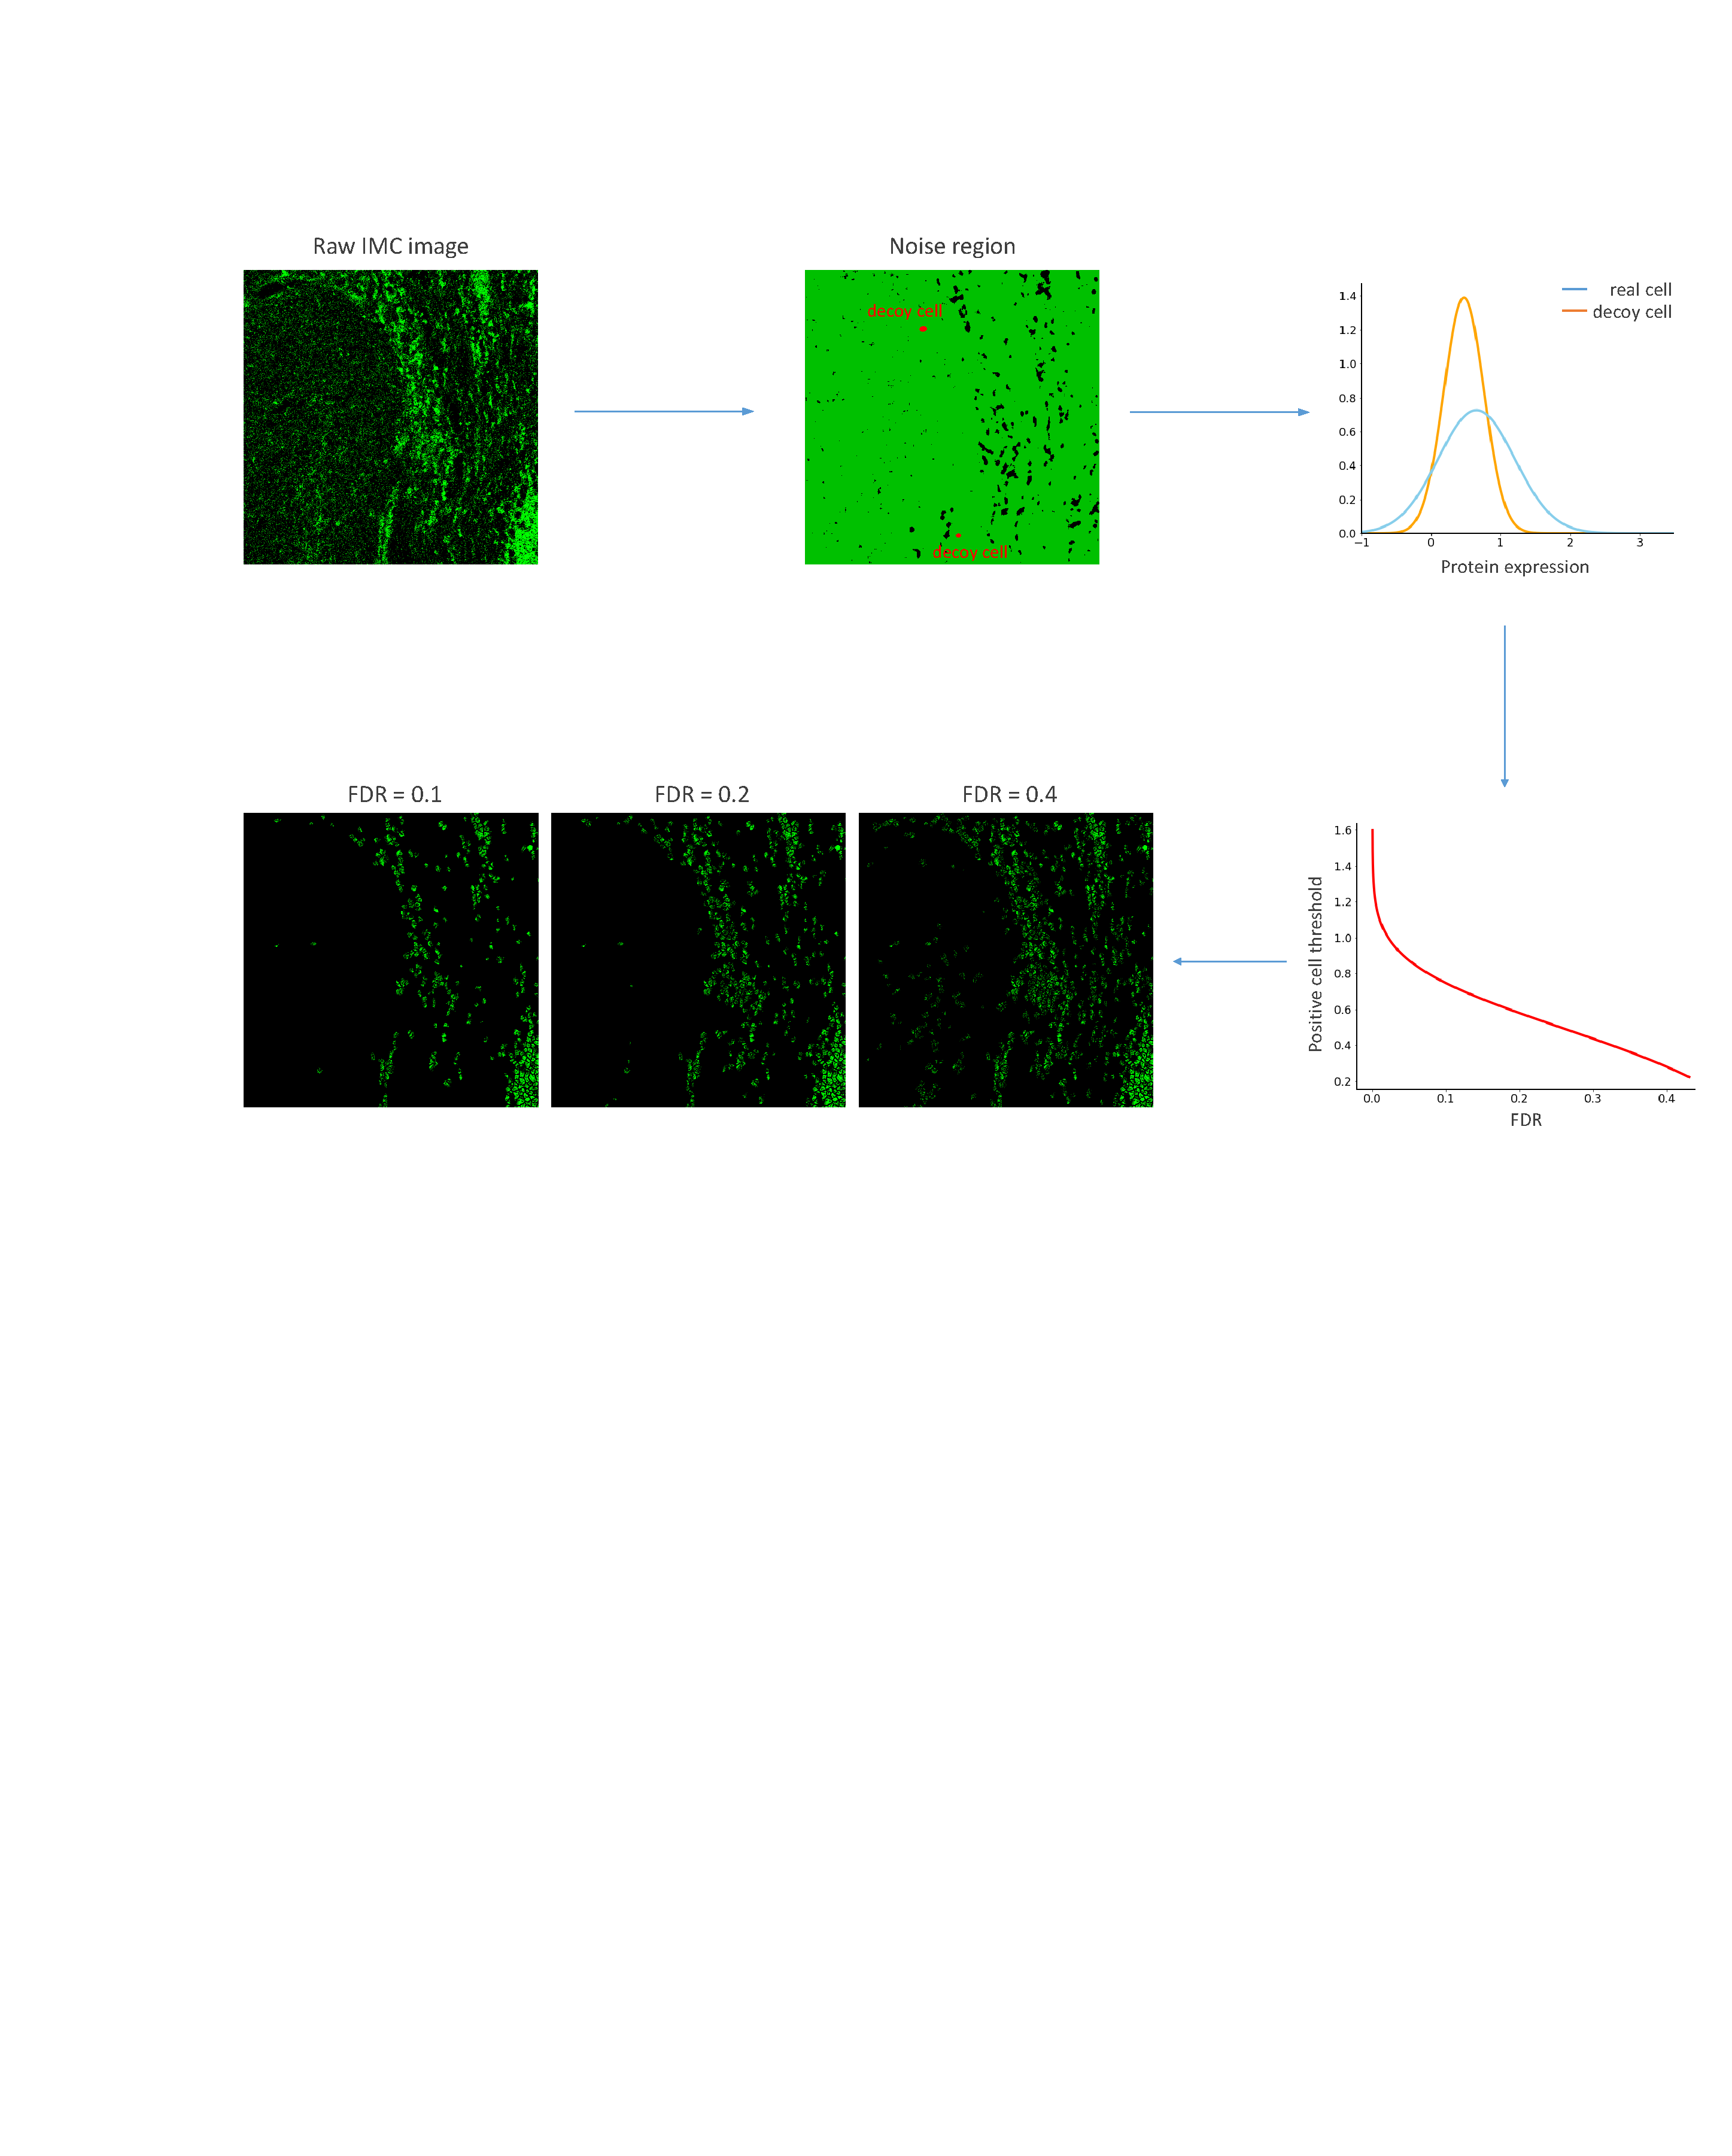
\includegraphics[width=\linewidth]{Figure/Figure4.pdf}
  \caption{Positive cells identified by IMCell with different FDR control (sample: 76 ROI18, protein: CD74). 
  }
  \label{fig4:pos}
\end{figure}


\begin{figure}[!htb]
  \centering
  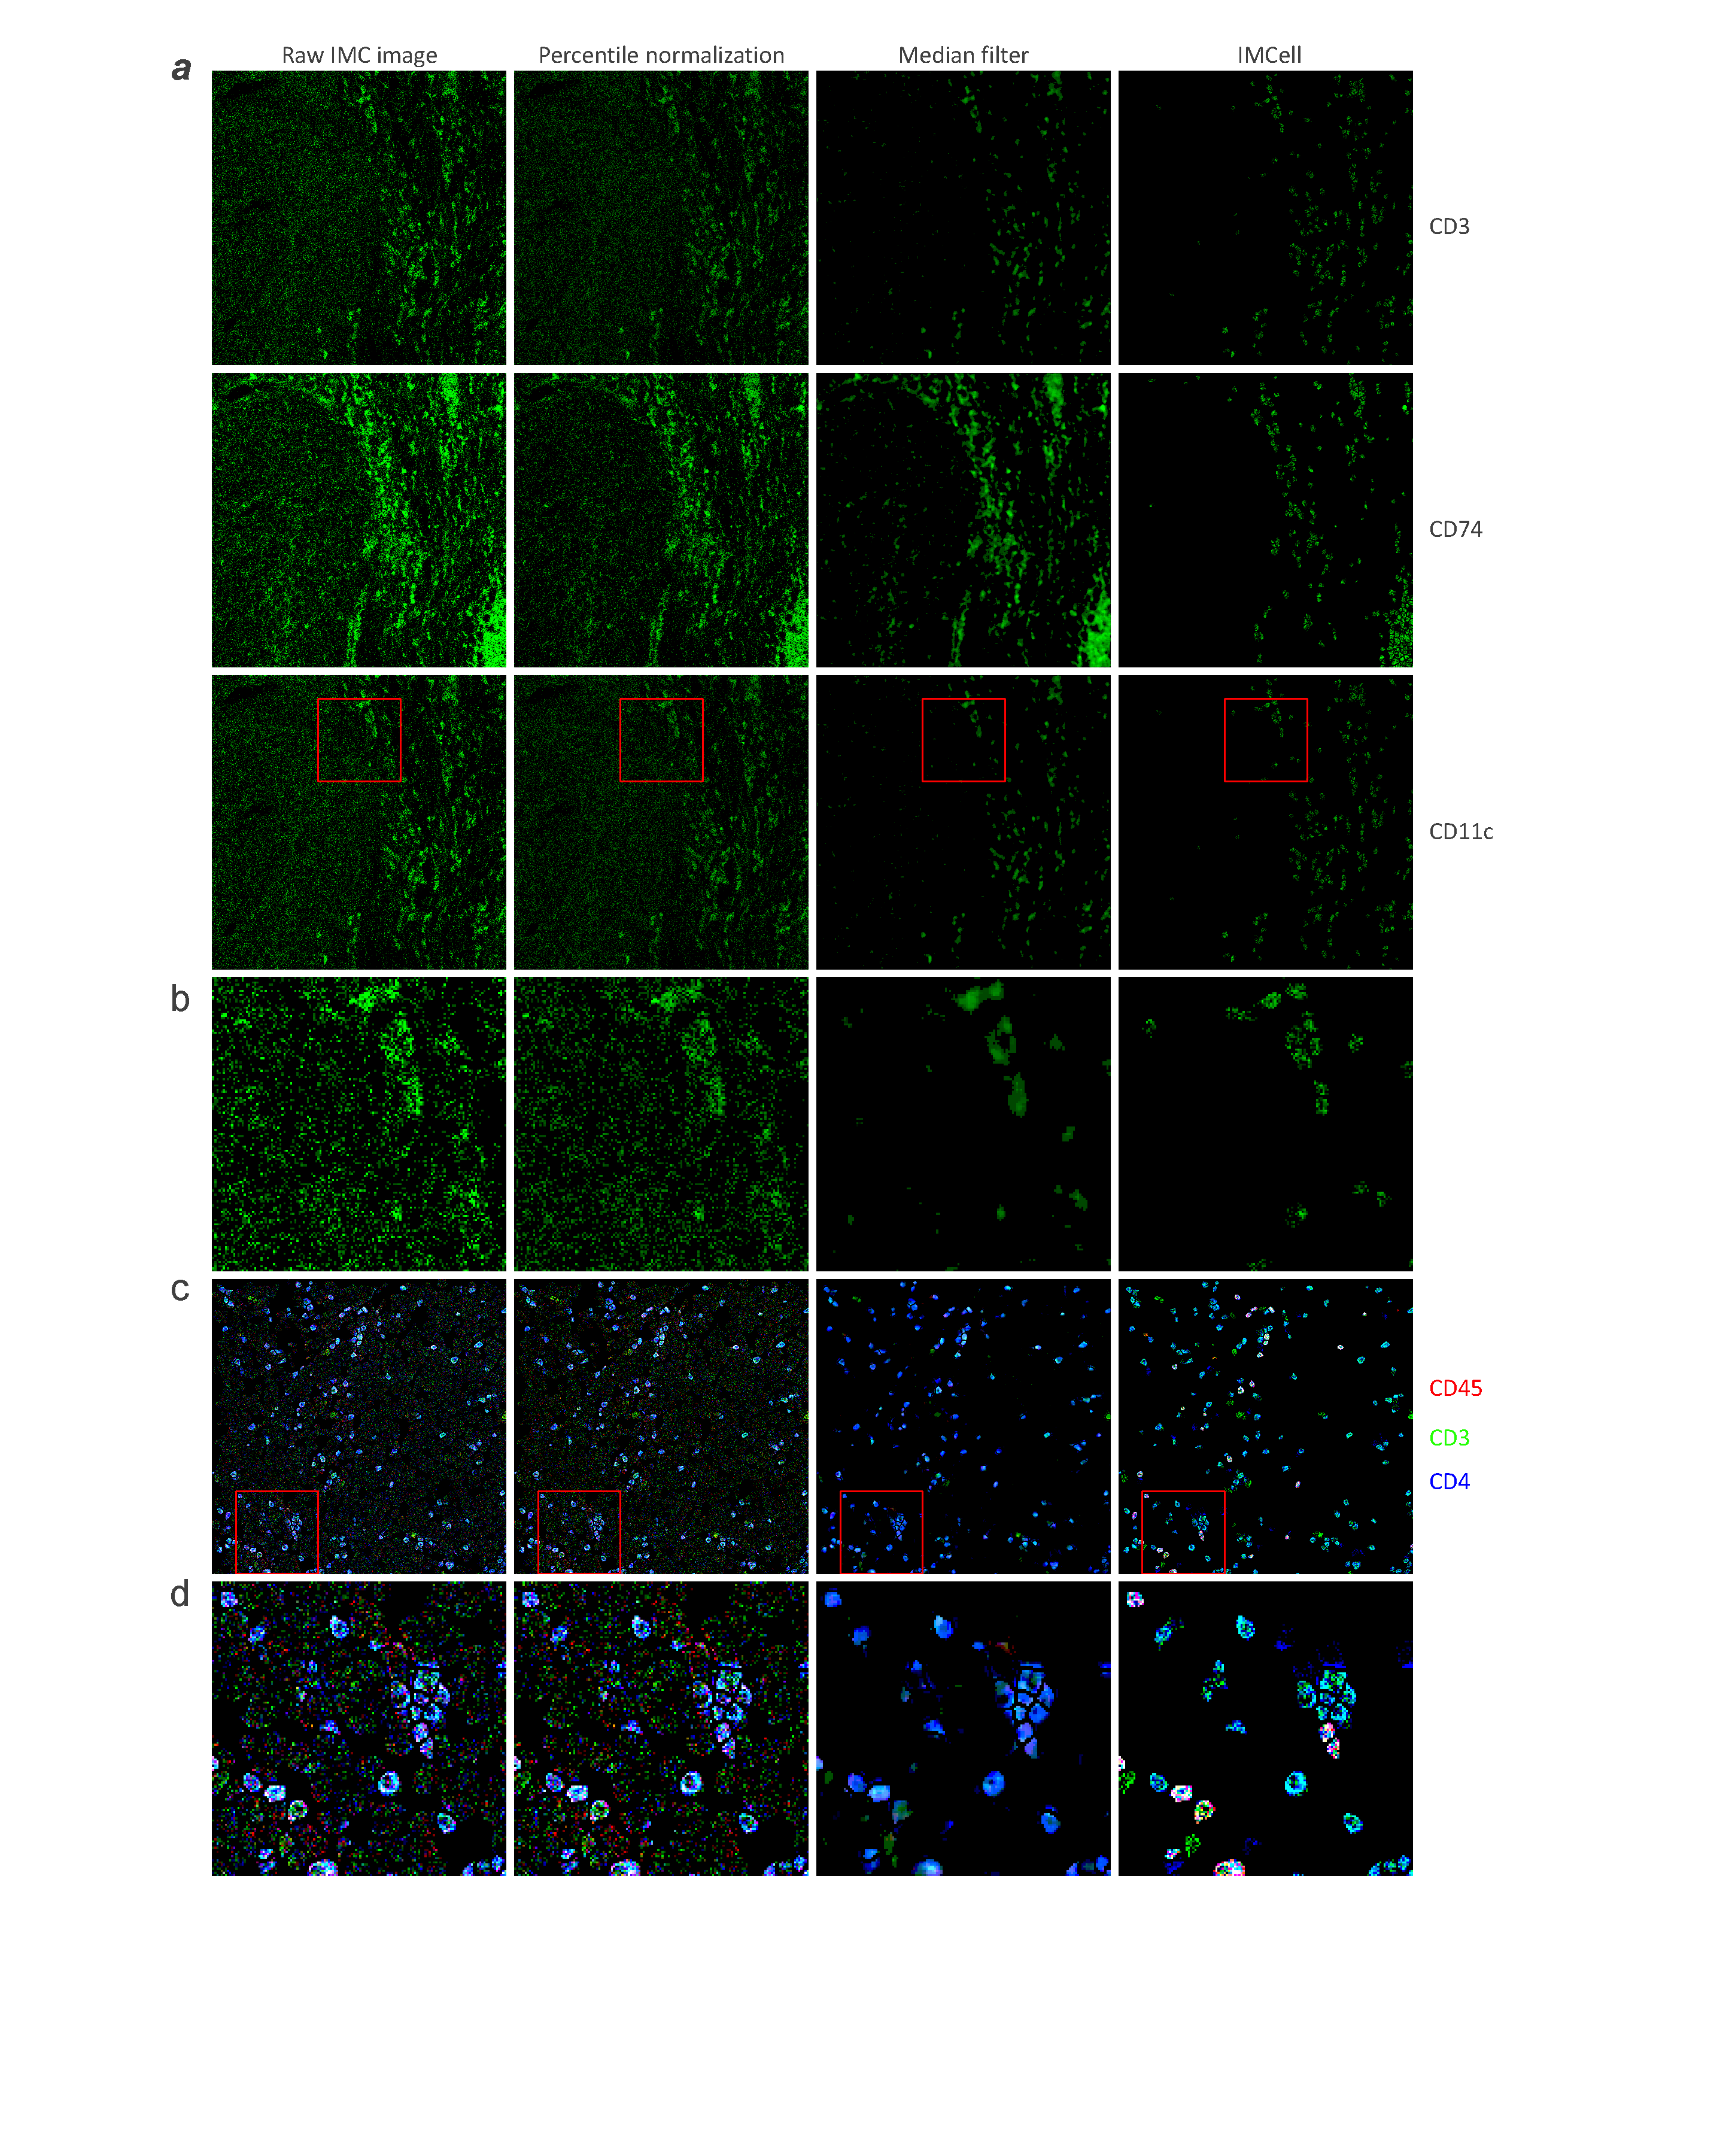
\includegraphics[width=0.9\linewidth]{Figure/Figure2.pdf}
  \caption{ Performance evaluation of different methods. 
  (a) Comparisons of cell identification results from raw IMC images, with $1^{st}$-$99^{th}$ percentile method to remove outliers, with median filter to remove salt-and-pepper noise, and with IMCell (sample: 76 ROI18). The red box marks the zoomed in areas on the below side (b) depicting the CD11c marker.
  Expression pattern of multi-markers (CD45, CD3, and CD4) in the whole images (c) and zoom-in areas (d). 
  }
  \label{fig2:imgs}
\end{figure}



\begin{figure}[!htb]
  \centering
  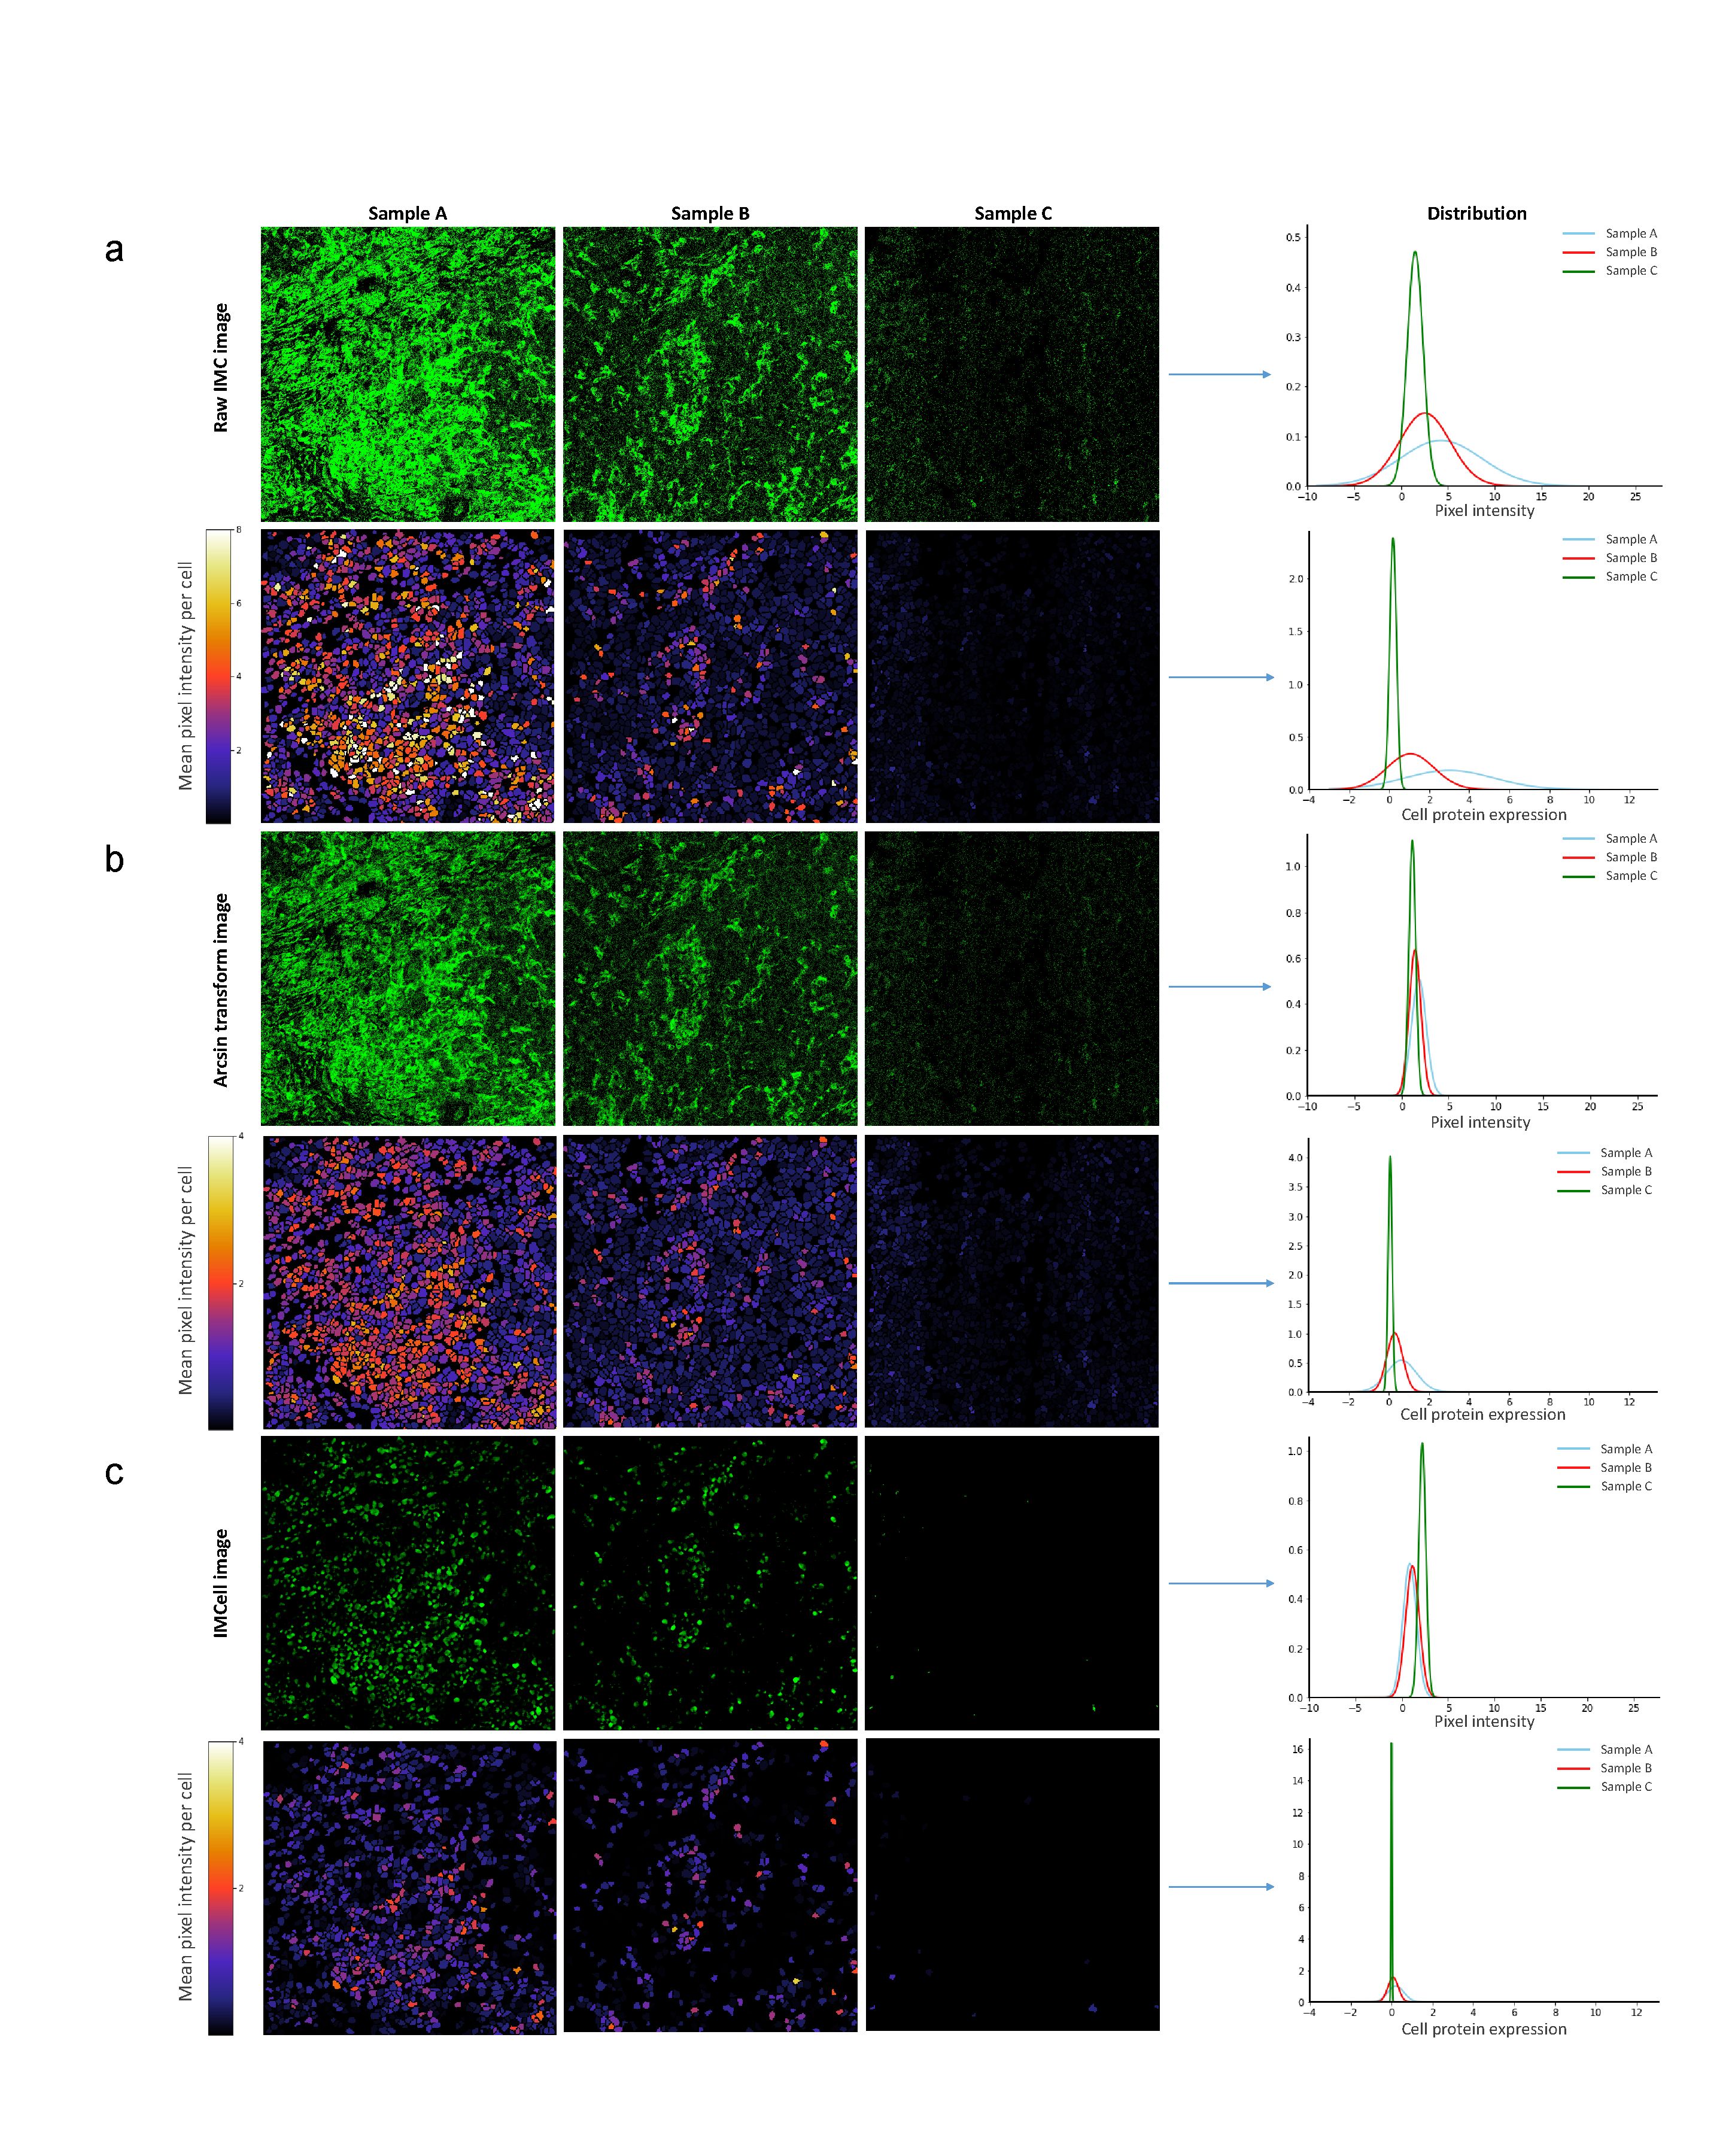
\includegraphics[width=0.9\linewidth]{Figure/Figure3.pdf}
  \caption{Variation of pixel intensity and cell protein expression across three samples (sample A: 65 ROI13, sample B: 65 ROI18, sample C: 33 ROI11). 
  The left column shows (a) the pixel intensity (first row) and cell protein expression (second row) from the raw images, (b) the pixel intensity (first row) and cell protein expression (second row) from arcsinh-transformed images, and (c) the pixel intensity (first row) and cell protein expression (second row) from images processed by IMCell. The right column plots the distribution of the corresponding value (i.e., pixel intensity and cell protein expression). 
  }
  \label{fig3:imcell}
\end{figure}



\begin{figure}[!htb]
  \centering
  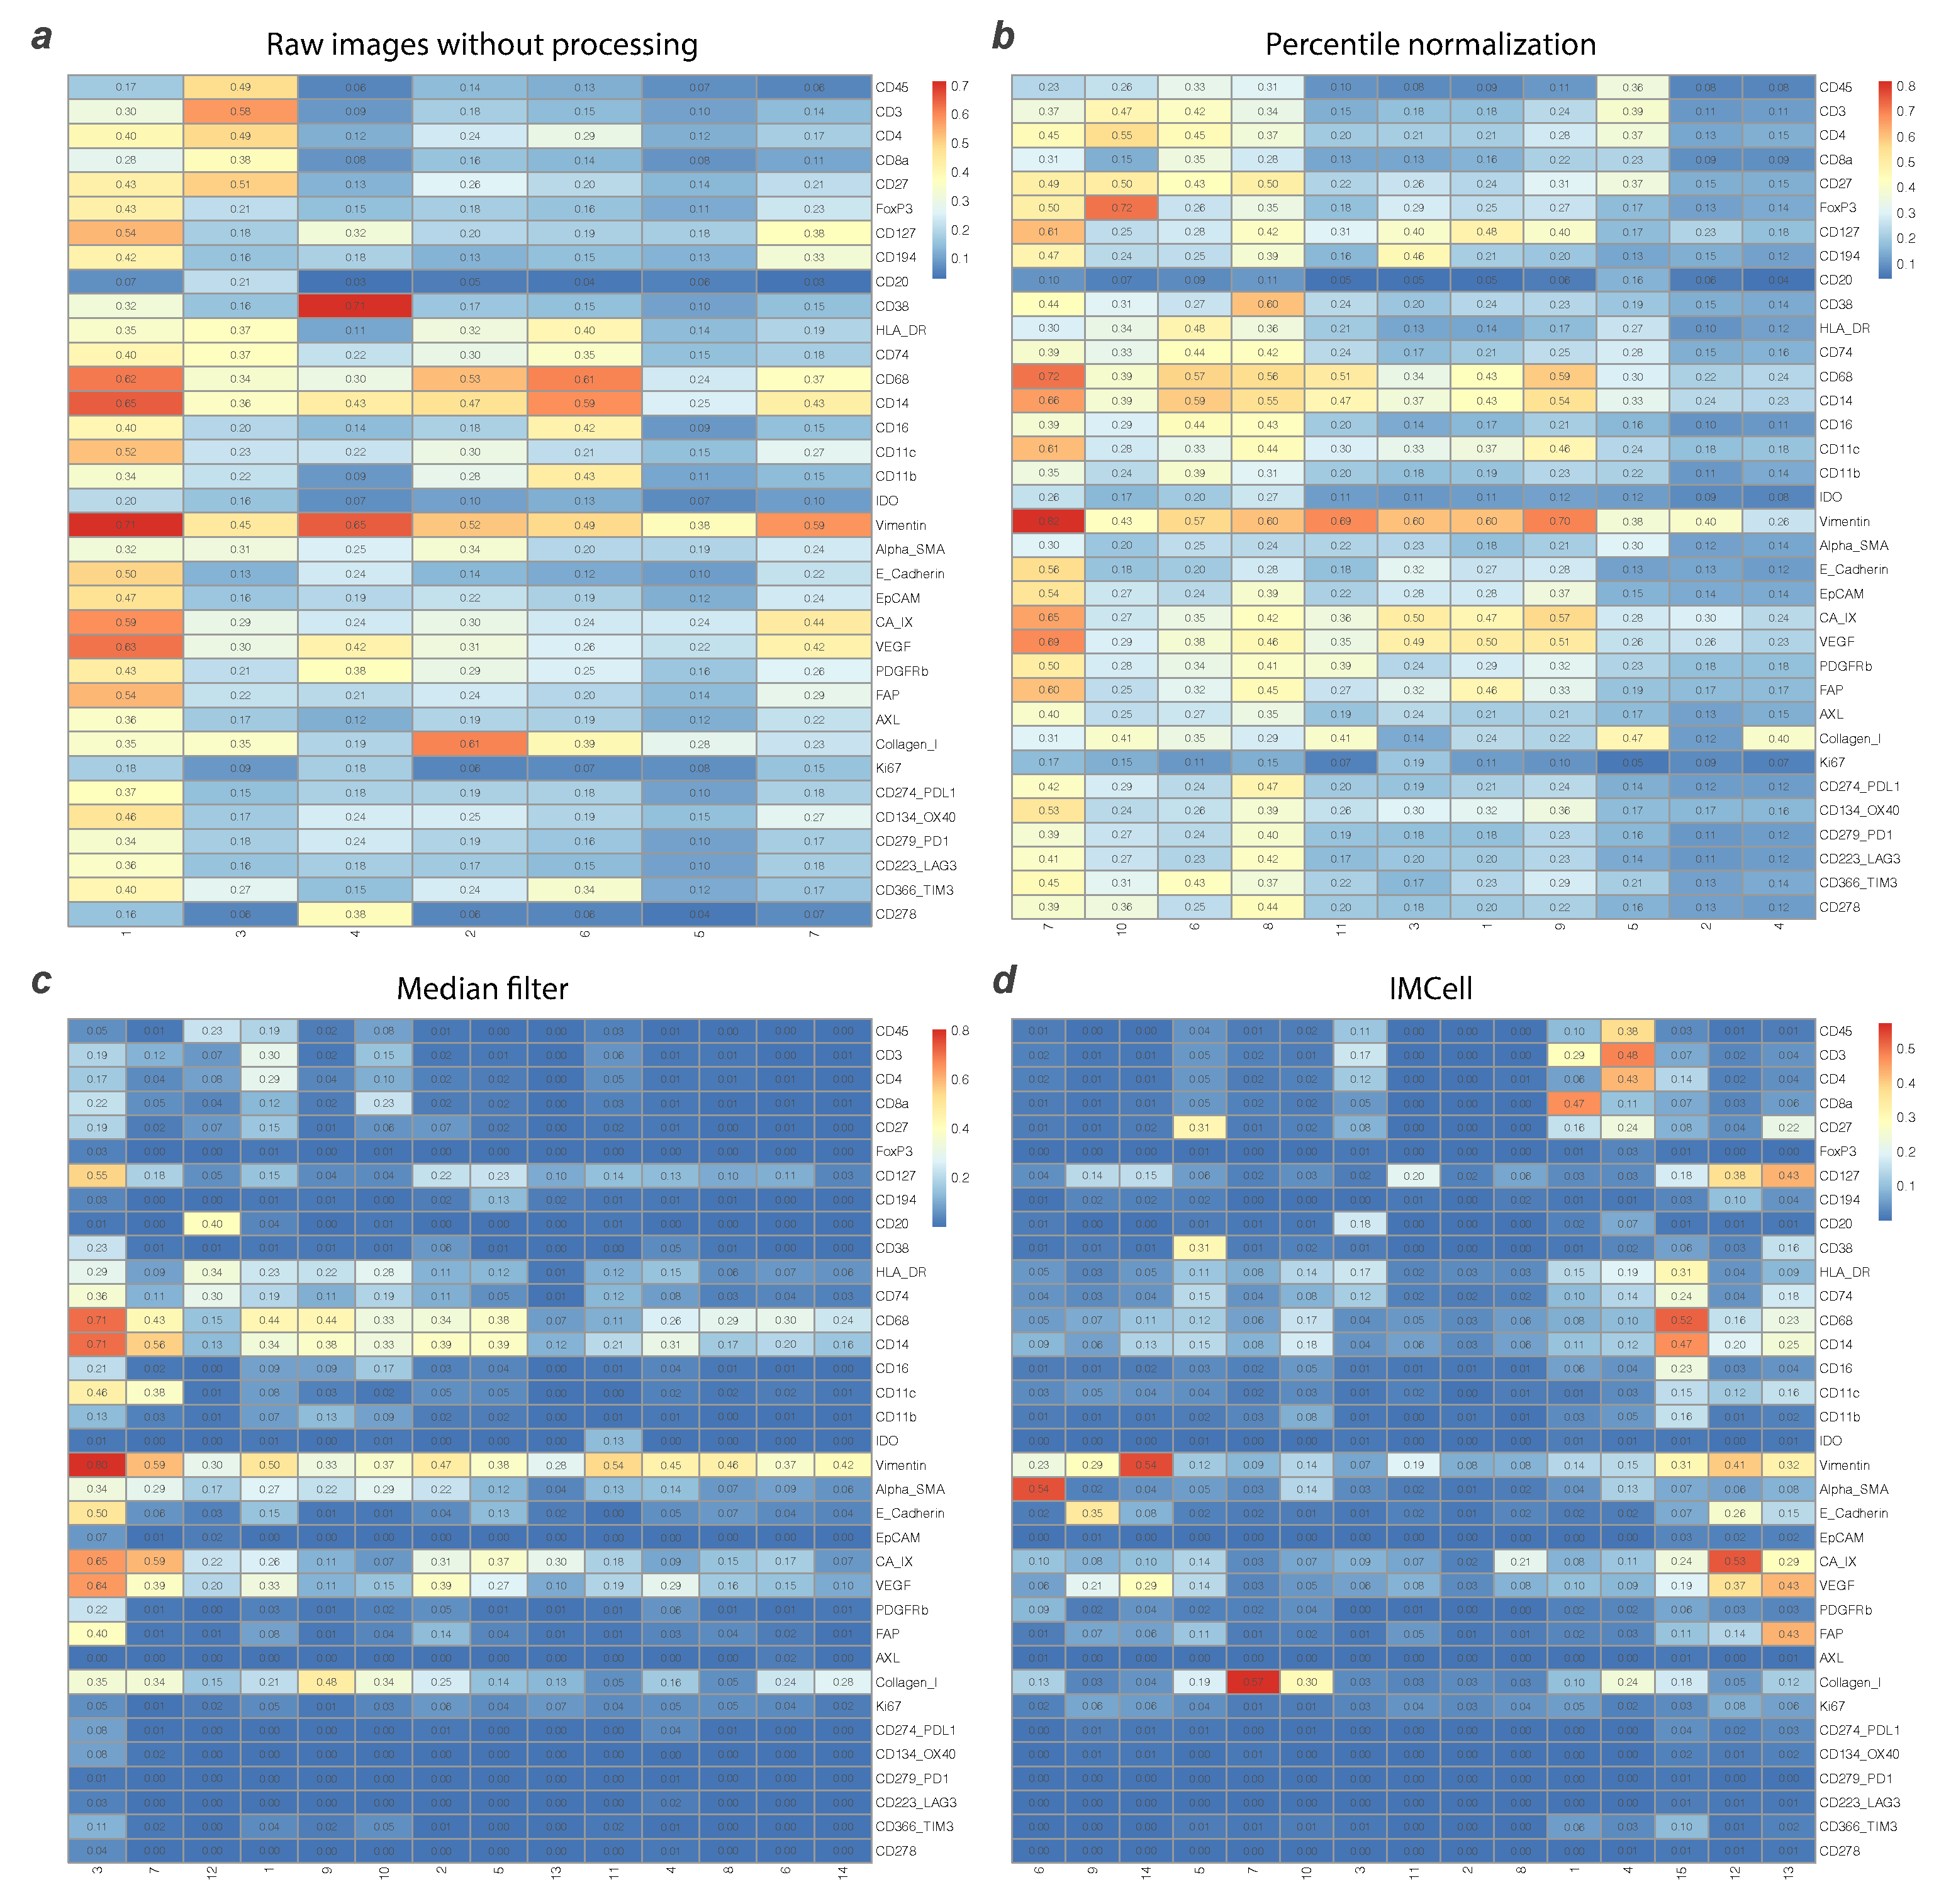
\includegraphics[width=\linewidth]{Figure/Figure5.pdf}
  \caption{Clustering result from different methods. Heatmap showing mean value of normalized protein expression in each cluster. The high-dimensional single cell expression data were generated from (a) raw IMC images, (b) with $1^{st}$-$99^{th}$ percentile method to remove outliers, (c) with median filter to remove salt-and-pepper noise, and (d) with IMCell. 
  }
  \label{fig5:cluster}
\end{figure}

\begin{figure}[!htb]
  \centering
  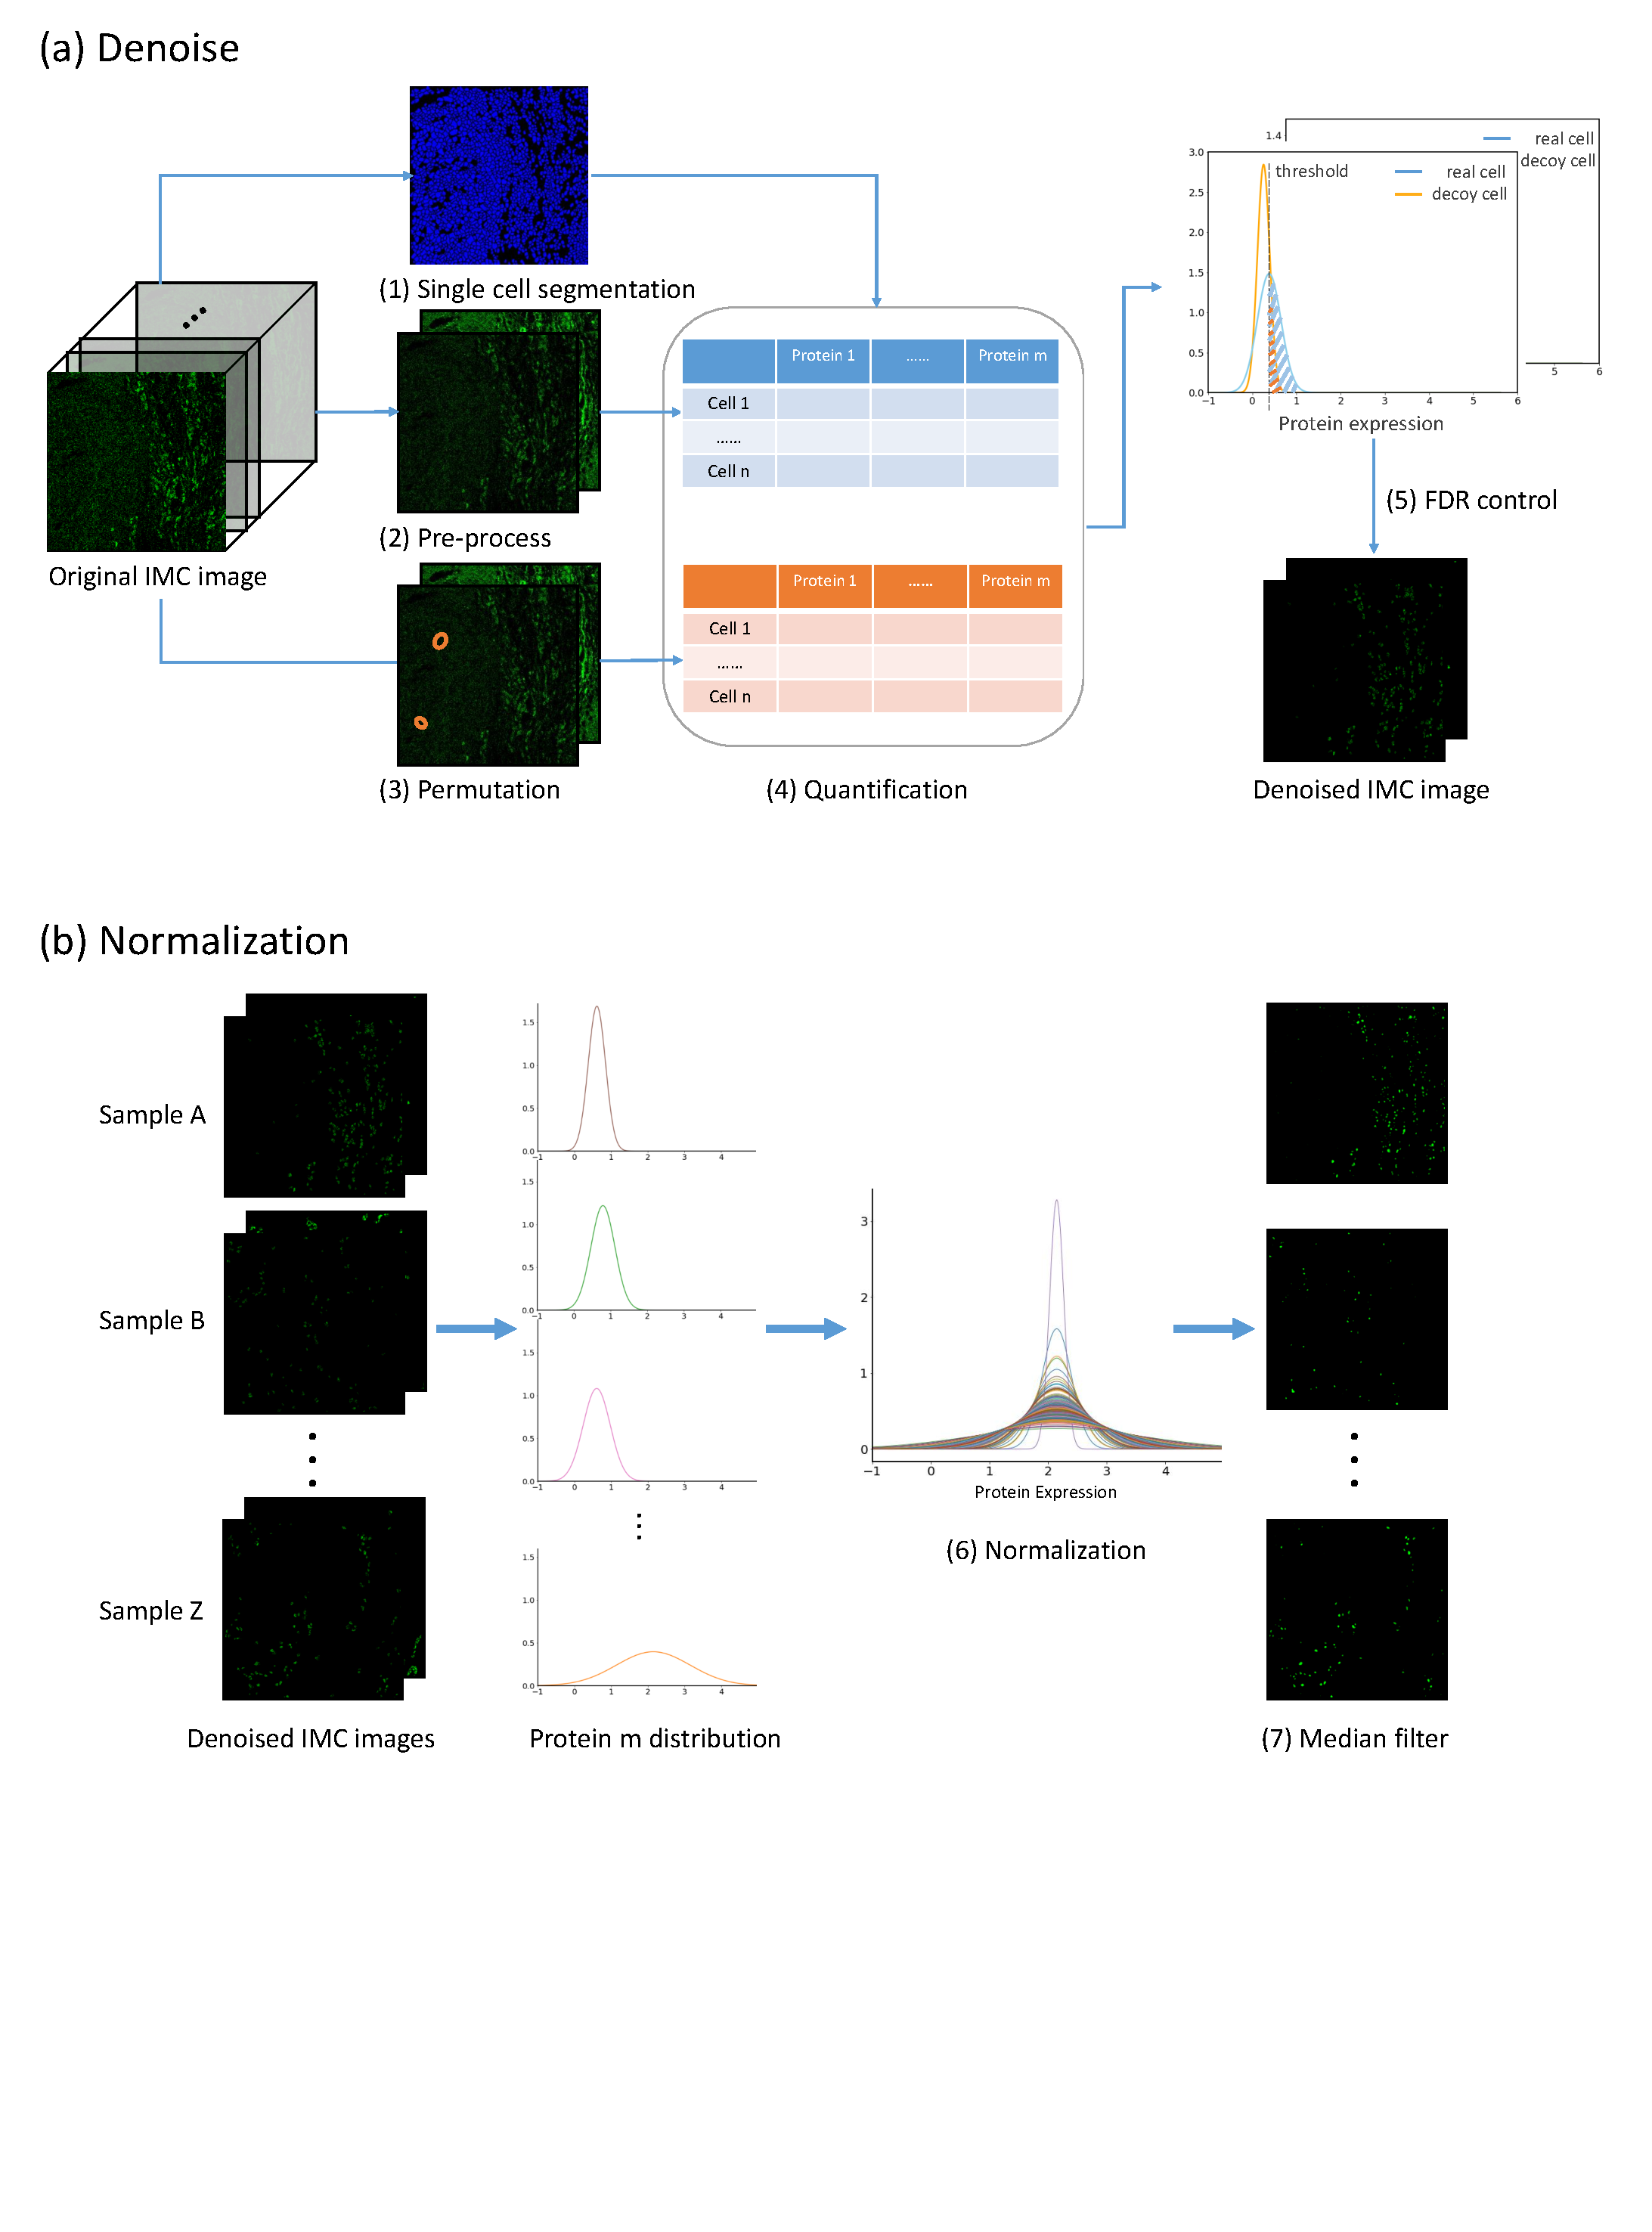
\includegraphics[width=\linewidth]{Figure/Figure1.pdf}
  \caption{The workflow of IMCell consists of (a) denoising and (b) normalization. The workflow includes the following procedures, (1) single cell segmentation by Dice-XMBD, (2) image pre-processing and hot pixel removal, (3) random generation of decoy cells in high-confidence noise regions, (4) protein quantification for segmented cells and decoy cells, (5) identifying positive cells with FDR control, (6) normalization by scaling using the mean of protein expression of positive cells, and (7) apply the median filter on the denoised and normlized images. 
  }
  \label{fig1:workflow}
\end{figure}



\end{document}
